
\documentclass[10pt]{article}

% amsmath package, useful for mathematical formulas
\usepackage{amsmath}
% amssymb package, useful for mathematical symbols
\usepackage{amssymb}

% graphicx package, useful for including eps and pdf graphics
% include graphics with the command \includegraphics
\usepackage{graphicx}

% cite package, to clean up citations in the main text. Do not remove.
\usepackage{cite}

\usepackage{color} 

% Use doublespacing - comment out for single spacing
%\usepackage{setspace} 
%\doublespacing


% Text layout
\topmargin 0.0cm
\oddsidemargin 0.5cm
\evensidemargin 0.5cm
\textwidth 16cm 
\textheight 21cm

% Bold the 'Figure #' in the caption and separate it with a period
% Captions will be left justified
\usepackage[labelfont=bf,labelsep=period,justification=raggedright]{caption}

\bibliographystyle{abbrv}

% Remove brackets from numbering in List of References
\makeatletter
\renewcommand{\@biblabel}[1]{\quad#1.}
\makeatother


% Leave date blank
\date{}

\pagestyle{myheadings}

\begin{document}

% Title must be 150 characters or less
\begin{flushleft}
{\Large
\textbf{The Effect of Uniqueness on Review Helpfulness}
}
% Insert Author names, affiliations and corresponding author email.
\\
Jack Hessel, 
Matthew Milano, 
Maithra Raghu
\end{flushleft}

\section*{Introduction}
What types of information are helpful to communities? The answer to this question undoubtedly depends on community type, size, and structure. Gilbert and Karahlios address this question in the Amazon review setting \cite{gilbert2010understanding} in the context of repetitive reviews. According to the authors, \emph{deja reviews} constitute ``missed opportunities'' because, when a user posts a review with little to no new content, ``the community [gains] little it did not already know.'' Their study includes interviews with amateur and experienced reviewers, and their findings indicate that, while amateur reviewers don't see the merit of a unique review, experienced reviewers take some personal pride in producing ``original'' content. They conclude with the suggestion that review sites should encourage amateur reviewers to produce unique content by ``[asking] for particular pieces of information.''

While it is clear that there is more unique information about the product contained in unique reviews, it is not obvious that unique reviews are truly more helpful and contribute more to review communities. For instance, it's plausible that a user, concerned with a primary feature of a product, would find an additional review echoing previous sentiments about that particular feature more helpful than a review about a secondary product feature she isn't interested in. Perhaps deja reviews, taken as a whole, are more helpful than reviews with unique content. This idea motivated our research question, ``are unique reviews \emph{actually} considered more helpful?''

Questions about how uniqueness relates to helpfulness have been addressed previously. For instance, Danescu-Niculescu-Mizil et al. find that reviews that give star ratings closer to the mean rating for the product are more likely to receive ``helpful'' votes on Amazon \cite{danescu2009opinions}. In their most successful model, Soo-Min et al. \cite{kim2006automatically} use a set of unigram tfidf features in an SVM regression to predict Amazon review helpfulness, indicating that lexical features do have an effect on helpfulness voting (though they do not report whether or not uniqueness had a positive or negative effect on helpfulness).

\section*{Data and Methods}
For our analysis, we use a dataset consisting of 500k Amazon ``fine foods'' reviews taken from 2002 to 2012 \cite{mcauley2013amateurs}. The information of interest contained in a given review includes the product ID to which it corresponds, the number of helpful/unhelpful votes it has received, and the text of that review. We restrict our consideration to 300 reviews in our dataset with the most total helpful votes, summed over all reviews of that product.

For each review, we remove all punctuation, capitalization, and map all numbers to a single token. Next, we create a vector space representation of a review using unigram tfidf features, where idf is computed with respect to a given product, rather than the whole dataset. This interpretation treats a given products' reviews as a corpus. Stemmed tokens that appear less than 2 reviews or in more than 80 percent of the reviews for a given product are discarded.

Next, the high-dimensional sparse per-document vectors are projected to an optimal linear subspace of 100 dimensions using PCA. After the dimensionality reduction step, reviews are clustered using a modified k-means clustering algorithm. Because many clustering methods, including k-means, are highly sensitive to outliers (for instance, the k-means objective utilizes an $L_2$ norm, so points far from cluster centers are very influential) and our goal is to use clustering for outlier detection, we implemented a slightly modified version of k-means, \emph{constrained k-means}, that enforces a minimal number of points in each cluster

Given $k$, the number of desired clusters, and $0 < p < \frac{n}{100k}$, the minimum proportion of the data that must be in each cluster, constrained k-means returns a reasonable clustering of the data that satisfies these parameters. To ensure that clusters are ``big enough,'' the method begins by running normal k-means, and checking cluster size. If the data is spread properly with respect to $p$, that clustering is returned. Otherwise, (k+1)-means is executed, and the two clusters with the closest centers are merged to produce k-means. If the (k+1)-means + 1 merge fails as well, (k+2)-means + 2 merges is executed, and so on. In this way, constrained k means consists of two steps: a flat clustering step, and a hierarchical clustering step.

After executing constrained k-means, we assign a ``uniqueness'' score to each clustered review by finding the distance between its vector representation and the closest cluster center. Because we choose $k$ to be 10, the clustering process allows for 10 ``prototypical'' review types. If a review is far from each of the cluster centers, it is assigned a high uniqueness score.

Finally, for a given product, we run a logistic regression of uniqueness on a new binary value ``helpfulness.'' We say a review is helpful if it has at least one helpful vote and more than $60\%$ of its helpful votes are positive. We are interested, in particular, in the resulting logistic regression coefficient on helpfulness. If this coefficient is generally positive over all products in our dataset, we conclude that uniqueness positively influences helpfulness. Conversely, if this coefficient is generally negative, uniqueness is a negative predictor of helpfulness.

\section*{Results}
An interesting question to ask is how well our clustering scheme produces prototypical reviews, and what those reviews look like. Unfortunately, it is difficult to directly derive meaning from cluster centers, as the PCA projection to 100 dimensions removes feature meaning from the new vector space. However, it is possible to examine points assigned to each cluster and to determine words with high tfidf scores among those documents. For every review, we computed the top ten words associated with each cluster. For products with generally positive reviews, there were few apparent differences between clusters (see Table \ref{tab:clusterex}). However, it's possible that there are underlying patterns within this clustering not immediately obvious to a human reader; the ten prototypical reviews, while likely all positive, might highlight different aspects of the product.

\begin{table}[h]
\centering
\begin{tabular}{lllll}
Cluster 0 & Cluster 1 & Cluster 2 & ... & Cluster 9   \\
coconut   & coconut   & (NUM)     &     & coconut     \\
great     & cooking   & br        &     & dry         \\
hair      & great     & coconut   &     & good        \\
love      & oil       & face      &     & hair        \\
oil       & price     & hair      &     & moisturizer \\
skin      & product   & im        &     & oil         \\
smells    & skin      & ive       &     & product     \\
stuff     & taste     & oil       &     & really      \\
use       & use       & skin      &     & skin        \\
wonderful & uses      & use       &     & use           
\end{tabular}
\caption{Prototypical words for the clustering of ``Nature's Way Coconut Oil.'' It's unclear that they are any differences between clusters. The product has an average rating of 4.7/5 stars.}
\label{tab:clusterex}
\end{table}

On the other hand, for products with mixed reviews, it's clear that our clustering method detected at least some customer sentiment. For instance, cluster 2 and cluster 9 in Table \ref{tab:clusterex2} clearly illustrate our method's capacity to identify prototypical reviews with different sentiments.

\begin{table}[h]
\centering
\begin{tabular}{lllll}
Cluster 0 & Cluster 1 & Cluster 2 & ... & Cluster 9 \\
(NUM)     & (NUM)     & arent     &     & good      \\
br        & just      & bad       &     & great     \\
calories  & like      & fettucini &     & like      \\
cook      & maybe     & flavor    &     & love      \\
cooked    & miracle   & like      &     & noodles   \\
minutes   & noodles   & noodles   &     & pasta     \\
noodles   & product   & really    &     & product   \\
rinse     & texture   & rubbery   &     & really    \\
sauce     & tried     & texture   &     & taste     \\
water     & try       & wasnt     &     & (NUM)    
\end{tabular}
\caption{Prototypical words for the clustering of ``Miracle Noodle Shirataki Angel Hair Pasta,'' a gluten free, diet pasta. It's clear that there are any differences between clusters. The product has an average rating of 3.6/5 stars.}
\label{tab:clusterex2}
\end{table}

Figure \ref{fig:result} contains our primary findings. After analyzing the coefficient on uniqueness for each of the 300 product-level logistic regressions, we find that the average coefficient on uniqueness to be $-1.52$ ($p < 10^{-15}$). This is an indication that, based on our uniqueness and helpfulness metrics, lexical uniqueness has a negative influence on helpful voting. 

\begin{figure}[h!]
  \centering
  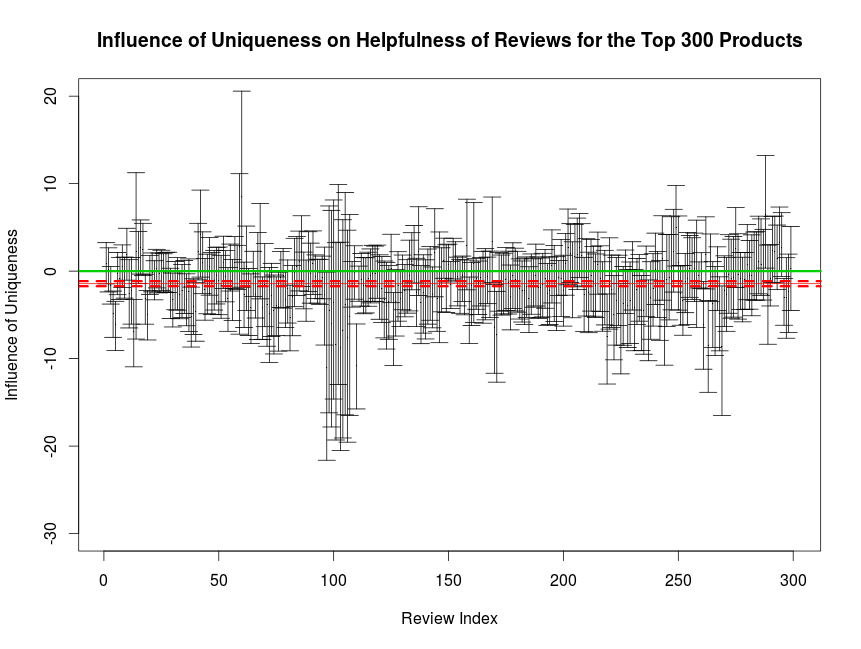
\includegraphics[width=0.8\textwidth]{influence.png}
  \caption{Document by uniqueness coefficient plot. For each of the top 300 documents, a logistic regression was executed, and the resulting coefficient with 95\% confidence intervals are demonstrated here. The red solid line indicates the mean coefficient, while the dotted red lines indicate 95\% confidence intervals on that value.}
  \label{fig:result}
\end{figure}

\subsection{Rating differences and Uniqueness}

The results so far indicate that uniqueness is perceived as not being helpful. One important factor for this might be that reviews that are more textually unique according to our analysis also rate the product differently from the majority of reviews. The lower score of helpfulness could then be readers disagreeing with the product rating, instead of the textual content of the review. 

We therefore reattempted logistic regression but with compensation for rating difference by subtracting the average rating of the product from the rating of the review that was being analysed. With this, the average coefficient did increase - becoming $-1.50$, but only very marginally. (The original value was $-1.52$.) This suggests that textual content perceived as different is still unhelpful to reviewers.


\section*{Conclusions}
Potentially in contrast to assumptions made by previous authors, we find that uniqueness is a negative predictor of review helpfulness. Though our methods are basic and could most definitely be improved upon, this preliminary result indicates that it is debatable as to whether or not unique reviews are truly more helpful to a community. We believe that the amount of useful information gained by repeating the same important idea again and again might outweigh the benefit of elaboration on secondary product features. We suspect this pattern emerges due to product simplicity. For instance, how many unique features of coconut oil require elaboration?

Notably, Mudambi et al. find that what makes a review helpful depends strongly on whether the product in question can be classified as a experience good, which cannot be truly evaluated until a consumer has \emph{experienced} it, or search good, which a customer can make most evaluations about prior to purchase \cite{mudambi2010makes}. Because our dataset consisted of the fine foods section of Amazon, most of the products in our dataset constitute experience goods. Consequently, our preliminary results might not extend to datasets that have higher proportions of search goods.

Finally, we recognize that our metric of uniqueness could be improved upon. For instance, it would be interesting to include bigram features in our vector space review representation. Also, our consideration is limited to extremely simple lexical review features only. A more complete analysis might include a subset of the dozens of more complex potential review features used by Ghose and Ipeirotis \cite{ghose2011estimating}. Our analysis also doesn't control for reviewer characteristics, which, given the complex social structure potentially underlying review sites like Amazon, is a potential avenue for future exploration.

\bibliography{refs}

\end{document}

